\documentclass[tikz,border=2pt]{standalone}
\usepackage{pgfplots}
\pgfplotsset{compat=1.18}
\usetikzlibrary{positioning}
\usepackage{helvet}
\renewcommand{\familydefault}{\sfdefault}
\definecolor{ieeecolor}{HTML}{042C53}
\definecolor{jrnlcolor}{HTML}{378ADD}
\definecolor{othercolor}{HTML}{B4B2A9}
\definecolor{confcolor}{HTML}{D98B3F}
\begin{document}
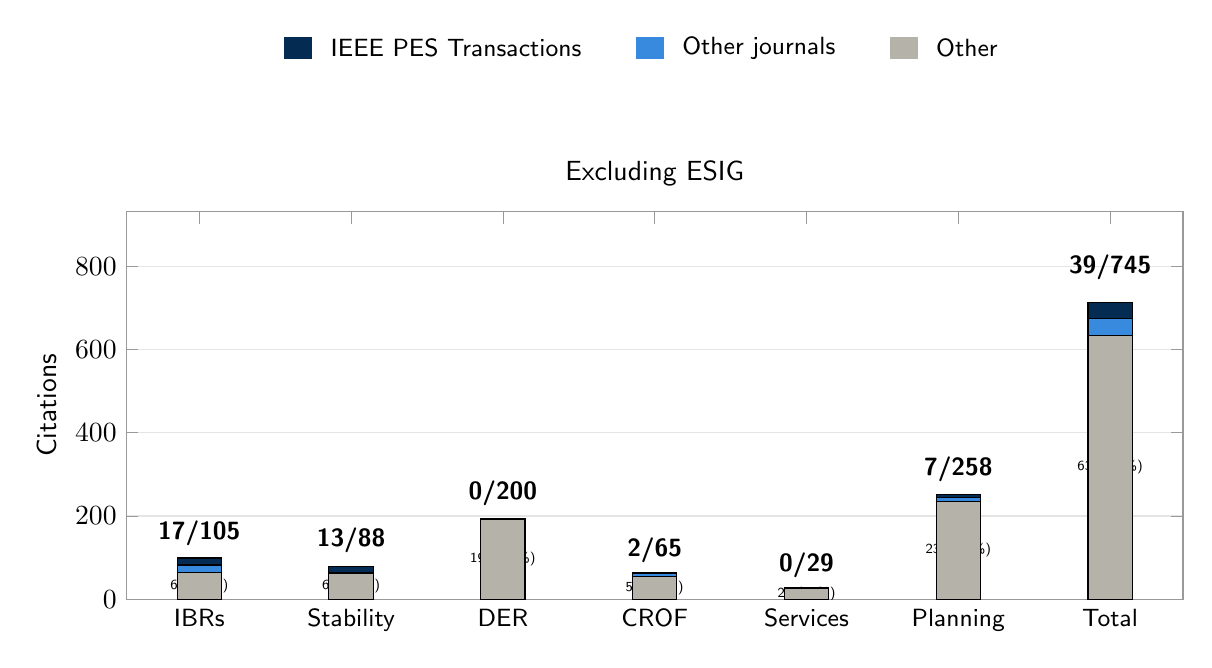
\begin{tikzpicture}
\begin{axis}[
    ybar stacked, bar width=16pt,
    width=15cm, height=6.5cm,
    symbolic x coords={IBRs,Stability,DER,CROF,Services,Planning,Total},
    xtick=data,
    x tick label style={font=\small},
    ylabel={Citations},
    ymin=0, ymax=931,
    axis line style={color=black!40},
    tick style={color=black!40},
    ymajorgrids, grid style={color=black!10},
    enlarge x limits=0.08,
    title={Excluding ESIG},
]
\addplot[fill=othercolor] coordinates {(IBRs,65) (Stability,62) (DER,192) (CROF,54) (Services,26) (Planning,235) (Total,634)};
\addplot[fill=jrnlcolor] coordinates {(IBRs,17) (Stability,3) (DER,2) (CROF,7) (Services,1) (Planning,10) (Total,40)};
\addplot[fill=ieeecolor] coordinates {(IBRs,17) (Stability,13) (DER,0) (CROF,2) (Services,0) (Planning,7) (Total,39)};
\node[font=\tiny, text=black] at (axis cs:IBRs,32.5) {65 (62\%)};
\node[font=\tiny, text=white] at (axis cs:IBRs,73.5) {17 (16\%)};
\node[font=\tiny, text=white] at (axis cs:IBRs,90.5) {17 (16\%)};
\node[font=\small\bfseries, anchor=south] at (axis cs:IBRs,105) {17/105};
\node[font=\tiny, text=black] at (axis cs:Stability,31.0) {62 (70\%)};
\node[font=\tiny, text=white] at (axis cs:Stability,71.5) {13 (15\%)};
\node[font=\small\bfseries, anchor=south] at (axis cs:Stability,88) {13/88};
\node[font=\tiny, text=black] at (axis cs:DER,96.0) {192 (96\%)};
\node[font=\small\bfseries, anchor=south] at (axis cs:DER,200) {0/200};
\node[font=\tiny, text=black] at (axis cs:CROF,27.0) {54 (83\%)};
\node[font=\tiny, text=white] at (axis cs:CROF,57.5) {7 (11\%)};
\node[font=\small\bfseries, anchor=south] at (axis cs:CROF,65) {2/65};
\node[font=\tiny, text=black] at (axis cs:Services,13.0) {26 (90\%)};
\node[font=\small\bfseries, anchor=south] at (axis cs:Services,29) {0/29};
\node[font=\tiny, text=black] at (axis cs:Planning,117.5) {235 (91\%)};
\node[font=\small\bfseries, anchor=south] at (axis cs:Planning,258) {7/258};
\node[font=\tiny, text=black] at (axis cs:Total,317.0) {634 (85\%)};
\node[font=\tiny, text=white] at (axis cs:Total,654.0) {40 (5\%)};
\node[font=\tiny, text=white] at (axis cs:Total,693.5) {39 (5\%)};
\node[font=\small\bfseries, anchor=south] at (axis cs:Total,745) {39/745};
\end{axis}
\begin{scope}[shift={(2.0,7.0)}]
\node[fill=ieeecolor, minimum width=10pt, minimum height=8pt, anchor=west] (legbox0) at (0,0) {}; \node[anchor=west, font=\small, right=3pt of legbox0] (legtxt0) {IEEE PES Transactions}; \node[fill=jrnlcolor, minimum width=10pt, minimum height=8pt, anchor=west, right=16pt of legtxt0] (legbox1) {}; \node[anchor=west, font=\small, right=3pt of legbox1] (legtxt1) {Other journals}; \node[fill=othercolor, minimum width=10pt, minimum height=8pt, anchor=west, right=16pt of legtxt1] (legbox2) {}; \node[anchor=west, font=\small, right=3pt of legbox2] (legtxt2) {Other};
\end{scope}
\end{tikzpicture}
\end{document}
